\section{Detectors cheatsheet}\label{sec:detectors-cheatsheet}

In the following figures, we show Pauli webs of all detectors in the unrepeated $X^1 Y^1 Z^1$ and $X^1 Z^1$ codes
and the repeated $X^2 Y^2 Z^2$ and $X^2 Z^2$ codes.

\newpage

\begin{figure}[p]
    \centering
    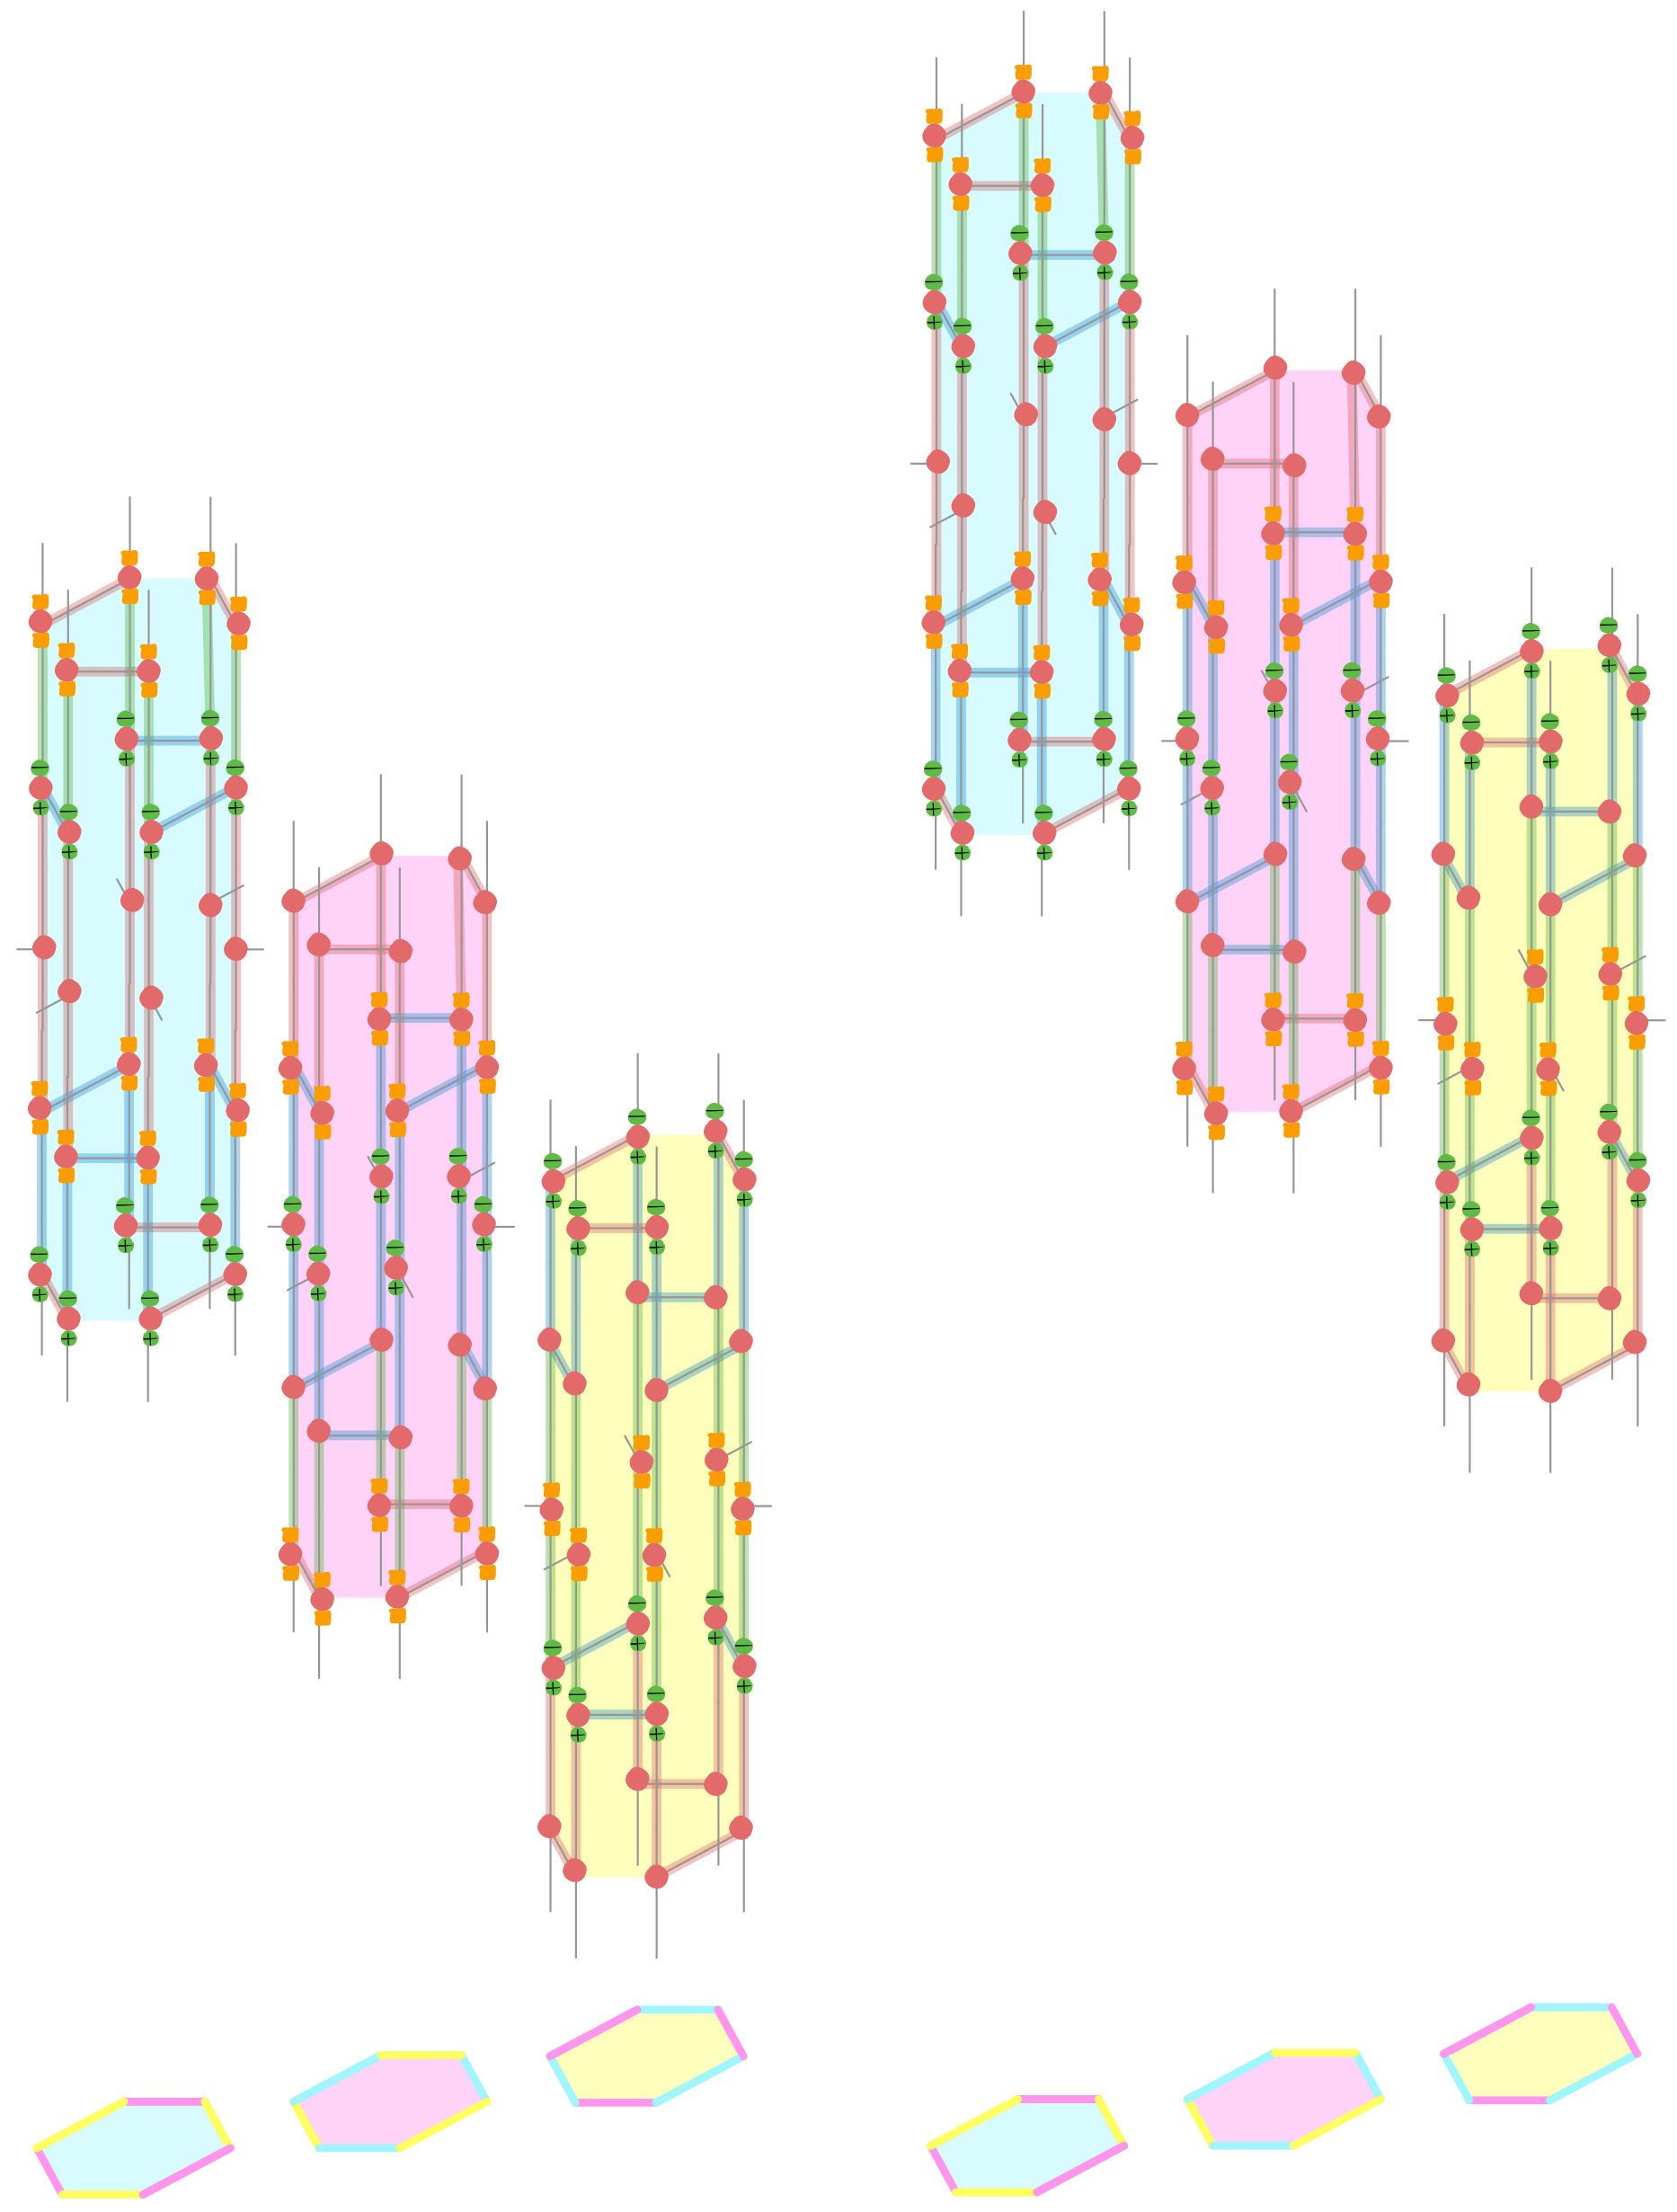
\includegraphics[width=\linewidth]{figures/detectors_reference/XYZ_all_detector_webs}
    \caption{$E$ (left) and $M$ (right) detectors of the $X^1 Y^1 Z^1$ code.}
    \label{fig:XYZ_all_detector_webs}
\end{figure}

\begin{figure}[p]
    \centering
    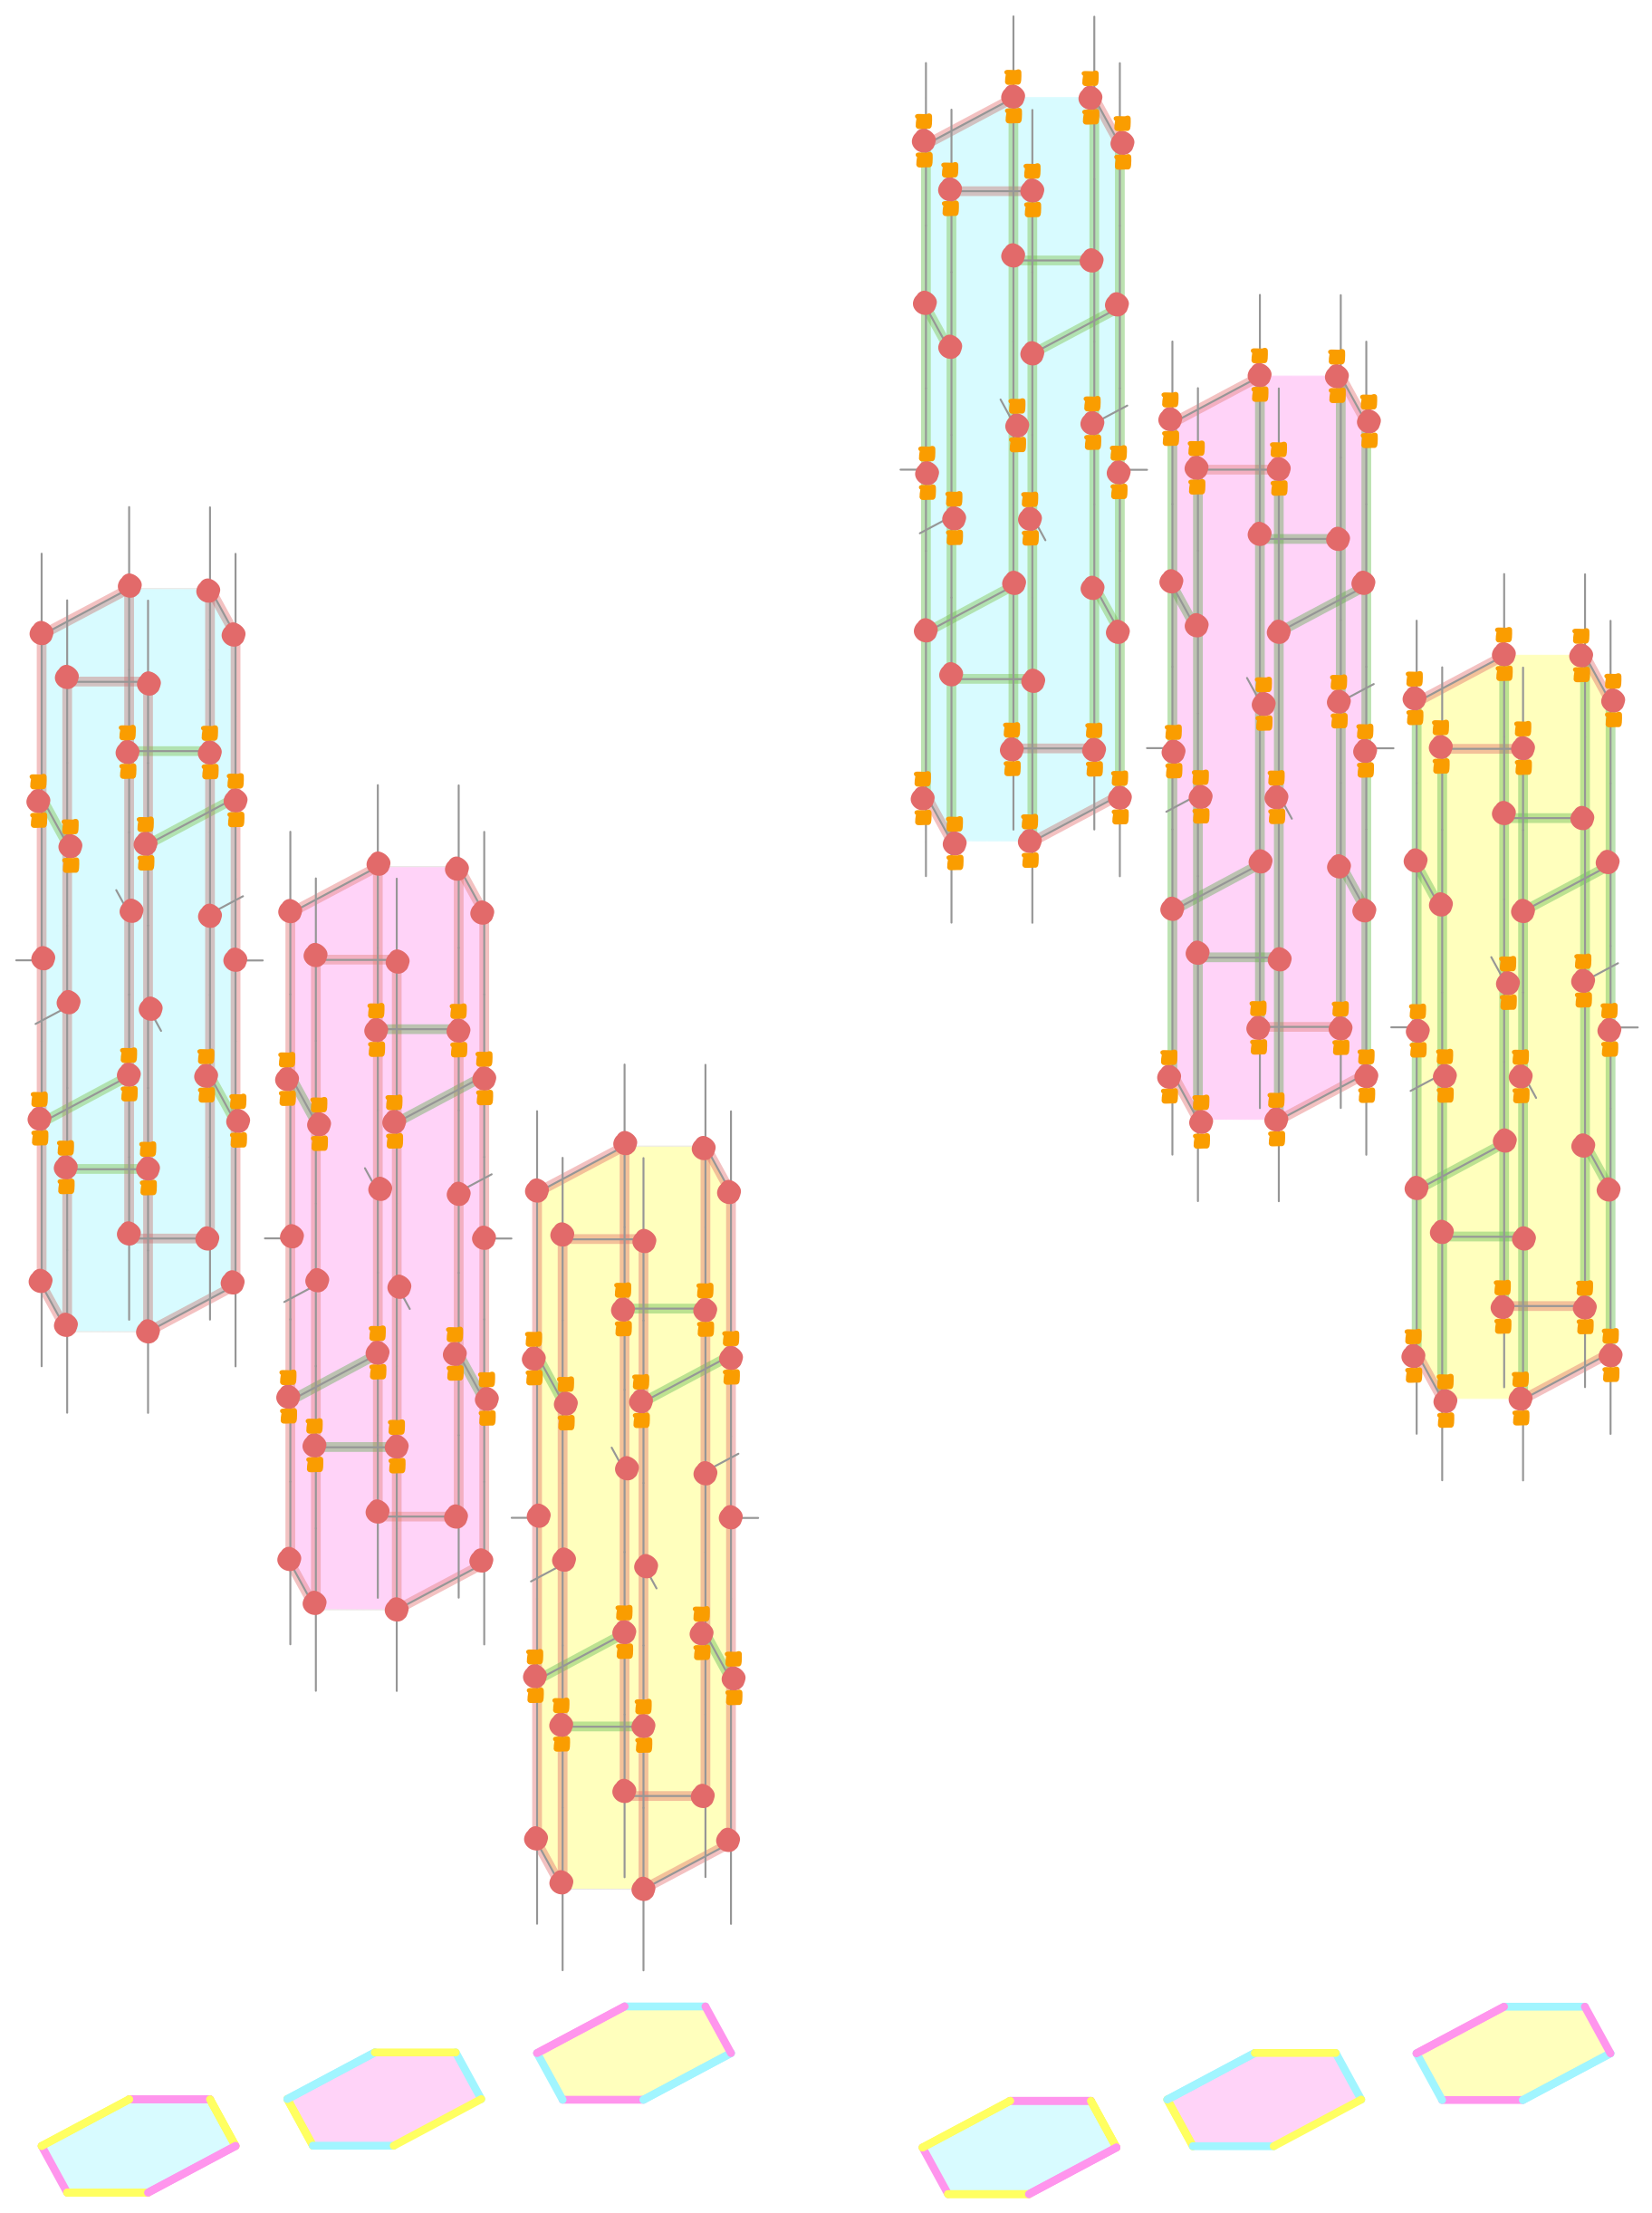
\includegraphics[width=\linewidth]{figures/detectors_reference/CSS_all_detector_webs}
    \caption{$E$ (left) and $M$ (right) detectors of the $X^1 Z^1$ code.}
    \label{fig:CSS_all_detector_webs}
\end{figure}

\begin{figure}[p]
    \centering
    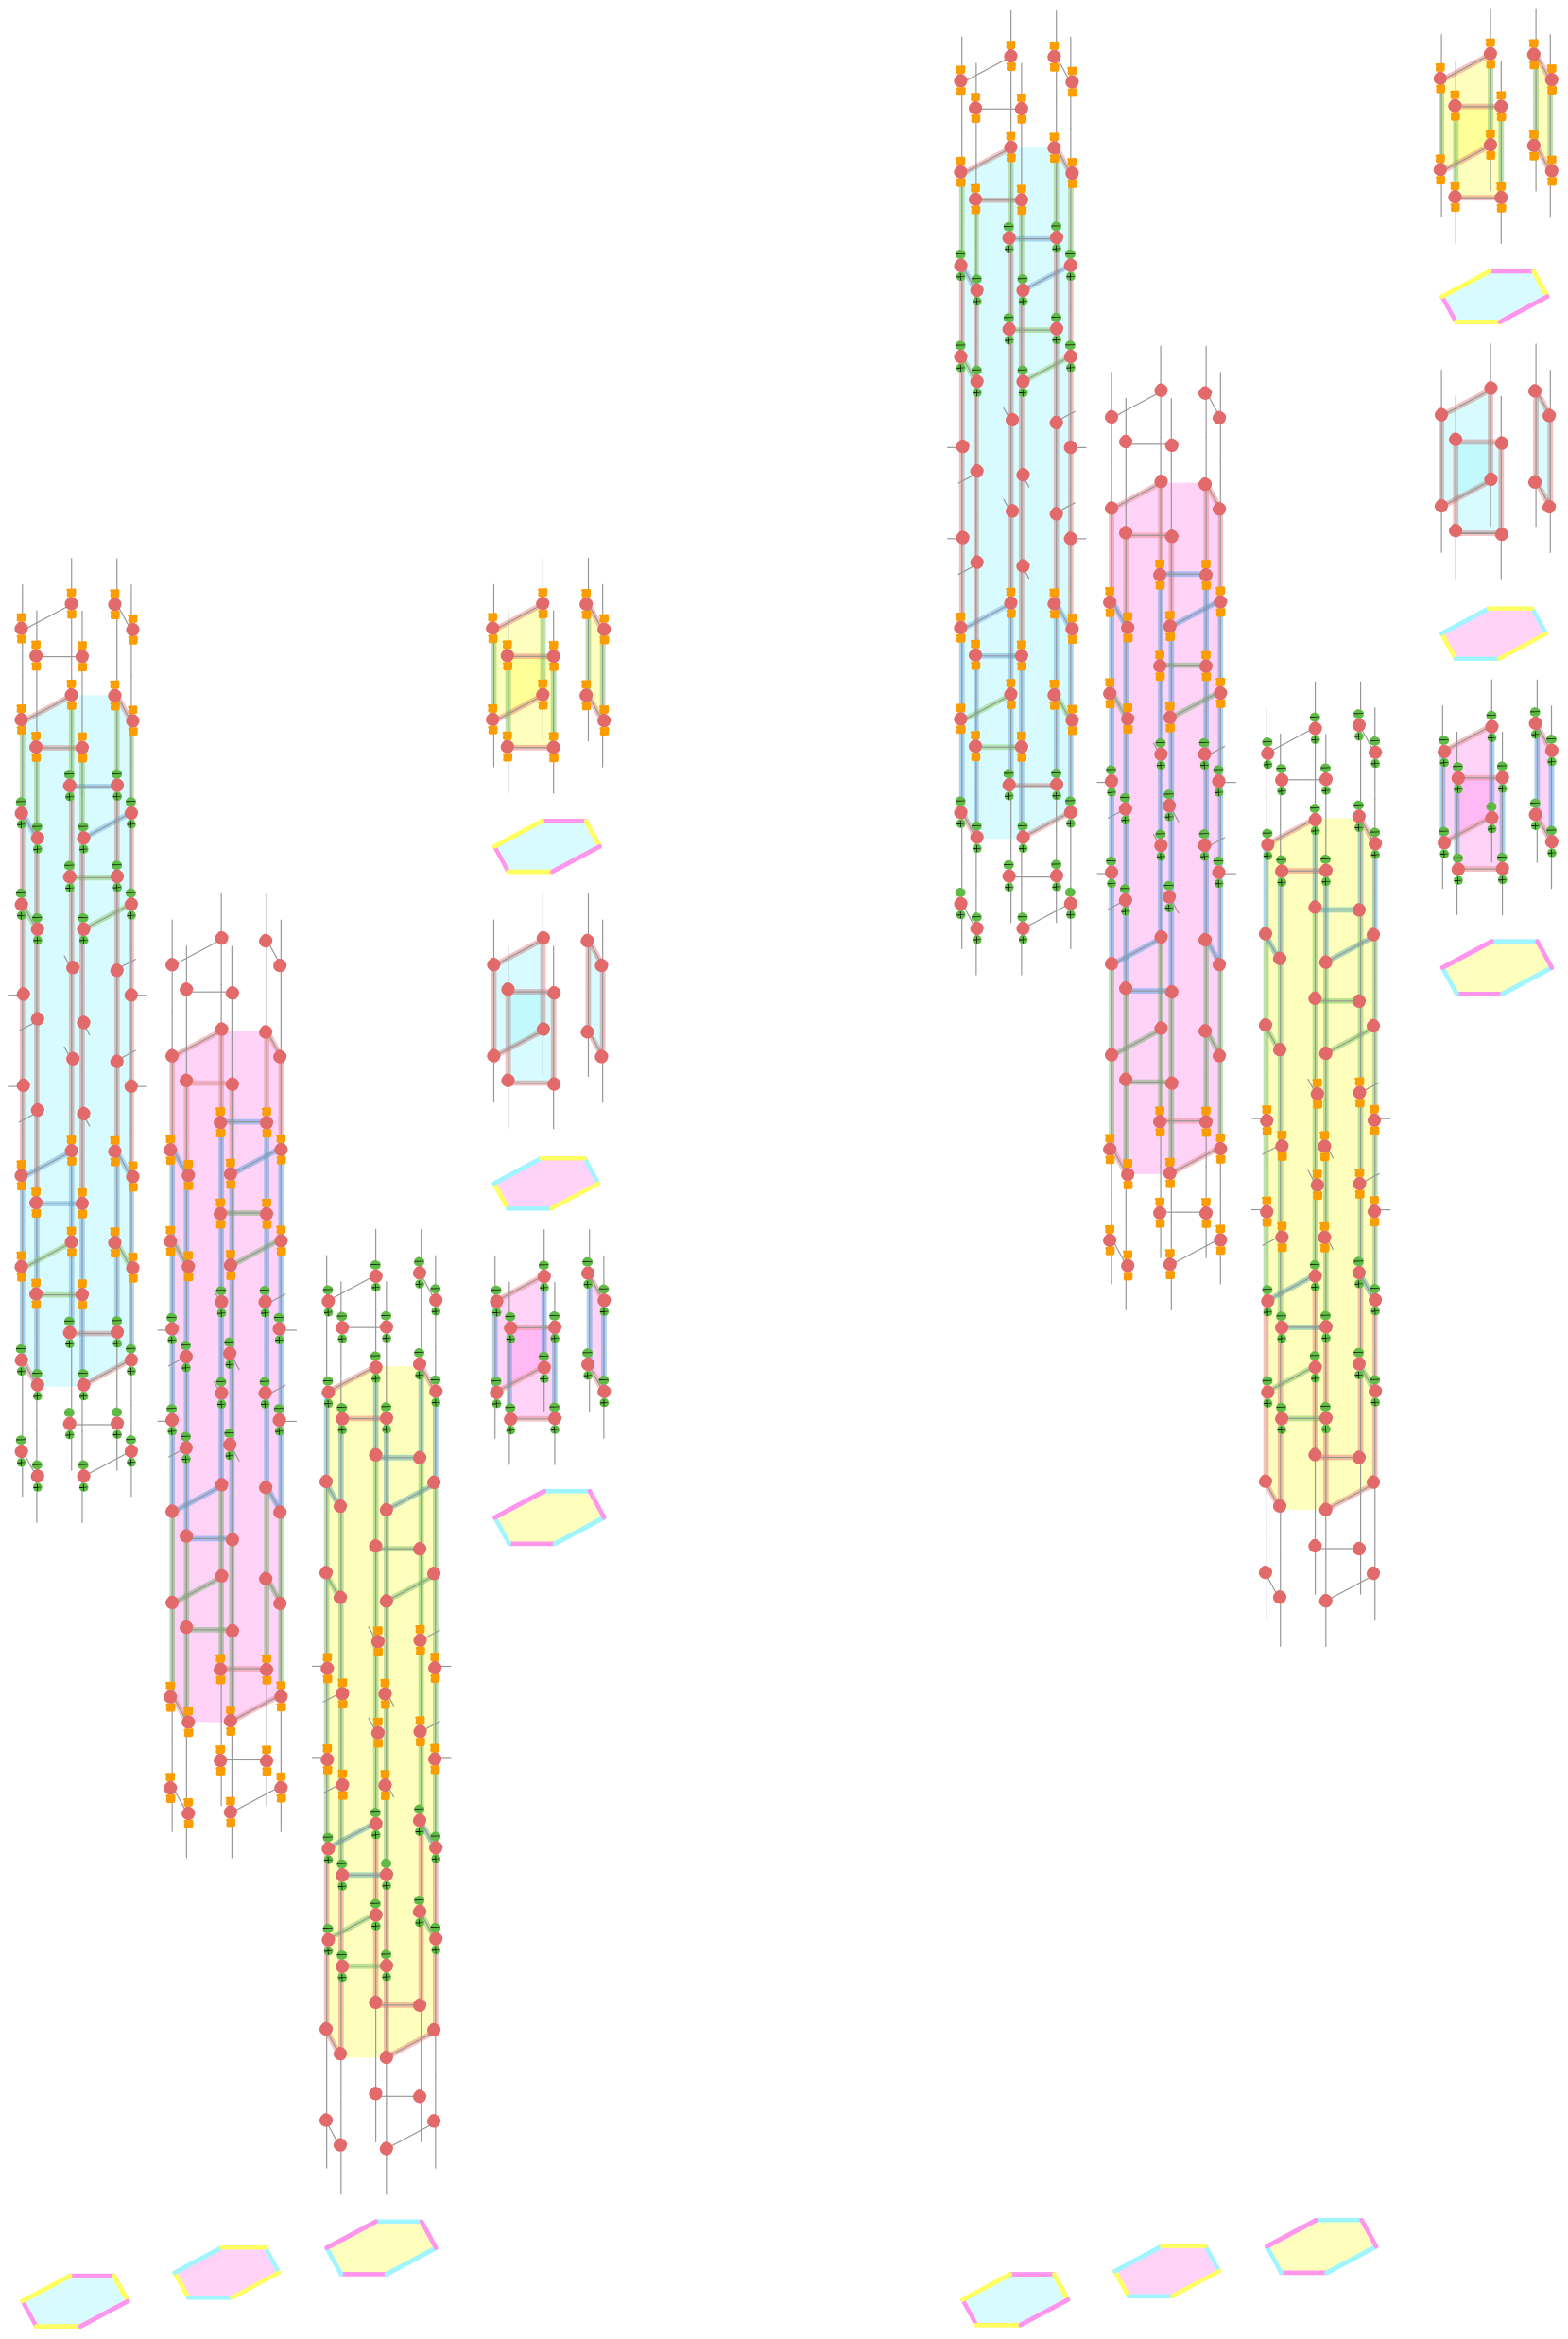
\includegraphics[height=0.95\textheight]{figures/detectors_reference/repeated_XYZ_all_detector_webs}
    \caption{$E$ (left) and $M$ (right) detectors of the $X^2 Y^2 Z^2$ code.}
    \label{fig:repeated_XYZ_all_detector_webs}
\end{figure}

\begin{figure}[p]
    \centering
    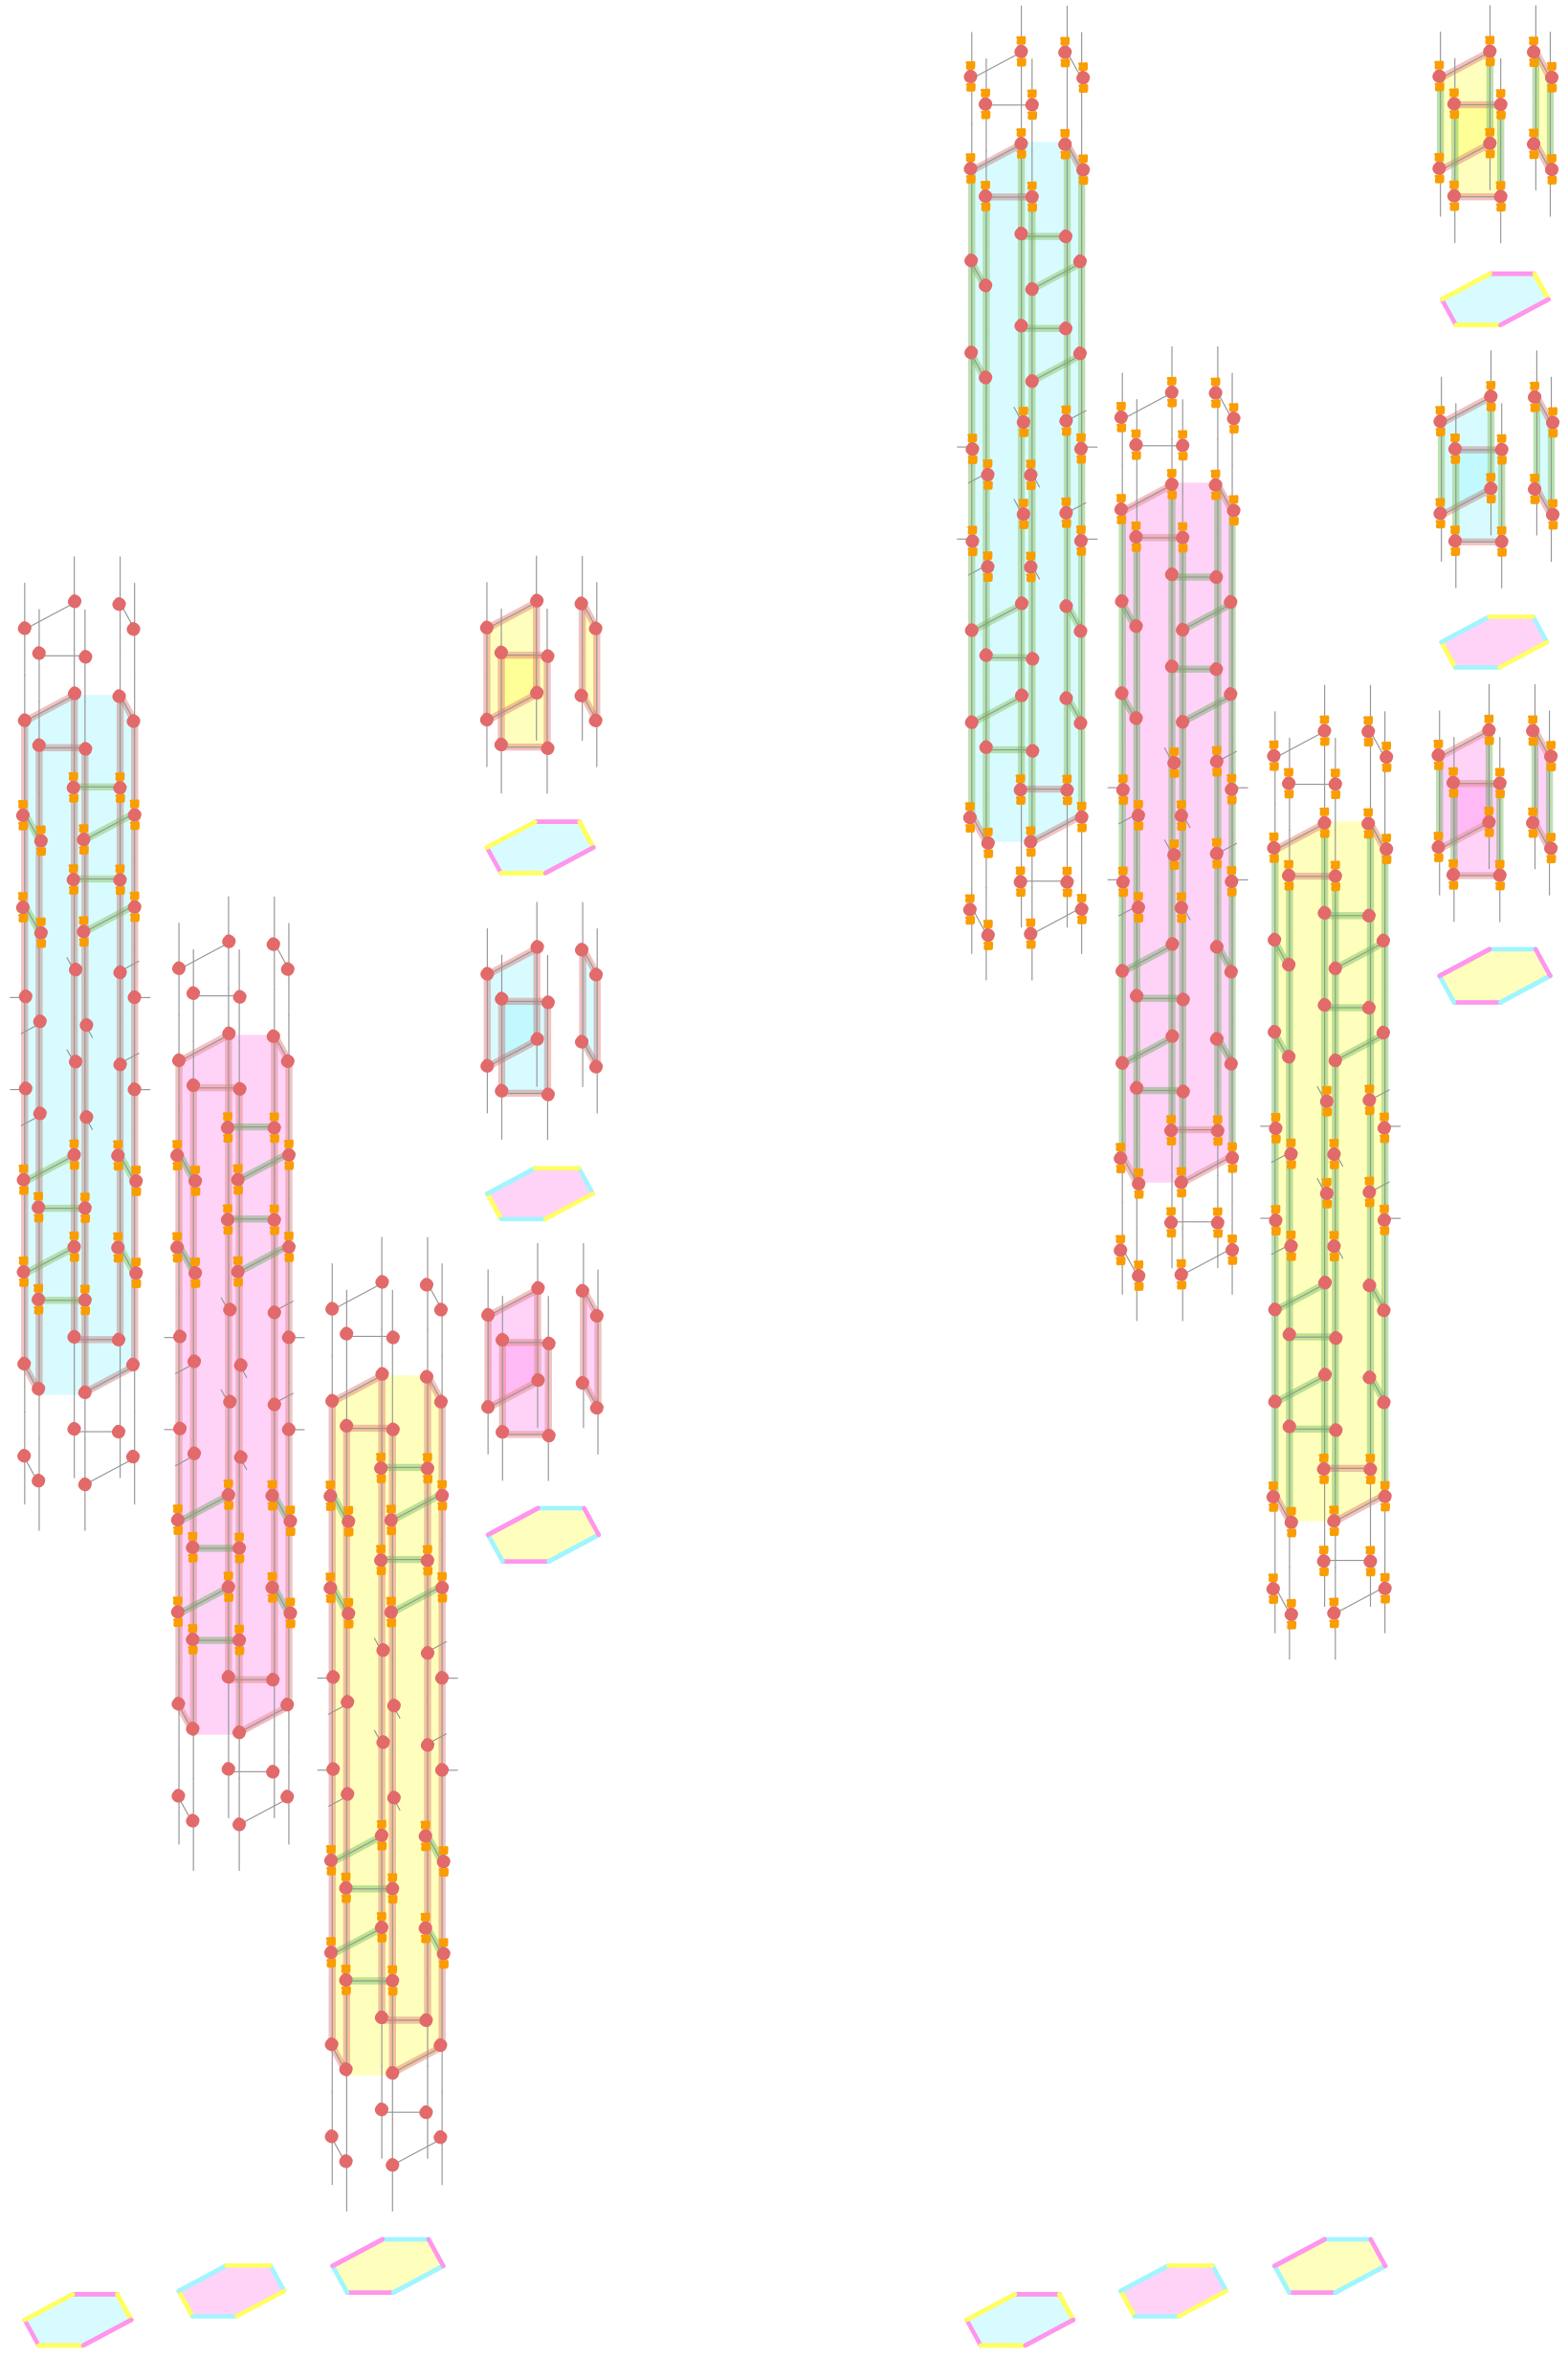
\includegraphics[height=0.95\textheight]{figures/detectors_reference/repeated_CSS_all_detector_webs}
    \caption{$E$ (left) and $M$ (right) detectors of the $X^2 Z^2$ code.}
    \label{fig:repeated_CSS_all_detector_webs}
\end{figure}


